\documentclass[a4paper, 12pt]{article}

\usepackage[T2A]{fontenc}
\usepackage[utf8]{inputenc}
\usepackage[english,russian]{babel}
\usepackage[left=15mm, top=20mm, right=15mm, bottom=20mm, nohead, nofoot]{geometry}

\usepackage{hyperref}
\usepackage{graphicx}
\usepackage{wrapfig}
\usepackage{afterpage}
\usepackage{amsmath, amsfonts, amssymb, amsthm, mathtools}
\author{Хомутов Андрей, группа Б06-903}
\title{ВПВ по курсу "Электричество и магнетизм" \\ Конденсатор на высоких частотах}
\date{22 декабря 2020 г.}
%%%%%%%%%%%%%%%%%%%%%%%%%%%%%%%%%%%%%%%%%%%%%%%%%%%%%%%%%%%%%%%%%%%%%%%%%
\usepackage{graphicx, wrapfig, subcaption, setspace, booktabs}
\usepackage[protrusion=true, expansion=true]{microtype}
\usepackage[english]{babel}
\usepackage{sectsty}
\usepackage{url, lipsum}
\newcommand{\HRule}[1]{\rule{\linewidth}{#1}}
\onehalfspacing
\setcounter{tocdepth}{5}
\setcounter{secnumdepth}{5}
%%%%%%%%%%%%%%%%%%%%%%%%%%%%%%%%%%%%%%%%%%%%%%%%%%%%%%%%%%%%%%%%%%%%%%%%%


\begin{document}

\title{ \normalsize \textsc{Лабораторная работа по физической химии}
		\\ [4.0cm]
		\HRule{0.5pt} \\ [0.3cm]
		\LARGE \textbf{{Определение ККМ в растворах ПАВ}}
		\HRule{0.5pt} \\ [0.1cm]
		\normalsize  \vspace*{18\baselineskip}}

\date{}

\author{Шамарина Екатерина, Б06-903 \\
		Хомутов Андрей, Б06-903 \\
ФБМФ, 2020\\ }

\maketitle
\thispagestyle{empty}
\newpage
%%%%%%%%%%%%%%%%%%%%%%%%%%%%%%%%%%%%%%%%%%%%%%%%%%%%%%%%%%%%%%%%%%%%%%%%%
\section*{Цели работы} 
\begin{enumerate}
    \item Освоение методик определения критической концентрации мицеллообразования ионогенных и неионогенных ПАВ по измерениям электропроводности и поверхностного натяжения растворов.
    \item Построение изотермы поверхностного натяжения и адсорбции ПАВ на поверхности раствор/воздух. Определение площади, занимаемой молекулой ПАВ в насыщенном адсорбционном слое.
    \item Оценка степени ионизации мицелл ионогенных ПАВ по результатам кондуктометрических измерений.
\end{enumerate}
%%%%%%%%%%%%%%%%%%%%%%%%%%%%%%%%%%%%%%%%%%%%%%%%%%%%%%%%%%%%%%%%%%%%%%%%%
\section{Теоретическая часть}
\subsection{Поверхностное натяжение}
В соответствии с уравнением адсорбции Гиббса зависимость коэфффициента поверхностного натяжения и примеси ПАВ в растворе задается следующим образом:
\begin{equation}
d \sigma=-\Gamma d \mu=-\Gamma \cdot R T \cdot d \ln c.
\end{equation}
Используя связь адсорбции и концентрации вещества через константу адсорбции можно получить уравнение Шишковского, описывающее эту кривую:
\begin{equation}
\sigma=\sigma_{0}-\Gamma_{\max } \cdot R T \cdot \ln (1+K c).
\end{equation}
Метод измерения поверхностного натяжения раствора ПАВ в этой работе представляет из себя метод пластинки Вильгельми. При достижении ККМ коэффициент поверхностного натяжения перестает падать и остается практически постоянным. Метод Вильгелми основан на изменении веса пластинки при свободном ее подвесе и при касании с жидкостью:
$$
\Delta \mathrm{F}=2 \sigma \cdot(d+L) \cdot \cos \Theta-\rho \cdot g \cdot x L d.
$$
Второе слагаемое отвечает за силу Архимеда, действующую на пластинку, погруженную в жидкость, а левое - за интересующую нас силу втягивания жикостью за счет поверхностного натяжения последней. Практически от влияния силы Архимеда можно избавиться за счет незначительного погружения пластинки в жидкость, а также за счет измерения силы при непосредственном отрыве ее от кромки воды. Фактически, в работе для этого измерялась максимальная сила, действующая на пластинку в процессе вытаскивания. От влияния угла смачивания тоже можно избавится, для этого материалом для пластинки должен хорошо смачиваться, эффект увеличивается за счет шероховатой поверхности.

В итоге можно достигнуть следующего удобного способа измерения поверхностного натяжения:
$$
\sigma=c\Delta \mathrm{F},
$$
где с - некоторая константа. 
\section{Практическая часть}
\subsection{Определение ККМ кондуктометрическим методом}
Для работы были приготовлены 13 растворов ПАВ (SDS c изначальной концентрацией 40 мМ), в диапазоне концентраций от 1/100 до 4 от ожидаемой ККМ с логарифмическим шагом, за исключением 13го раствора, концентрация которого была равна 8 мМ (ожидаемой ККМ). Объем каждого раствора - 25мл.
 
\begin{table}[h]
\begin{center}
\caption{Удельная электропроводность в зависимости от концентрации}
\begin{tabular}{|c|c|c|}
\hline
N раствора     & Cпав, мМоль  & $\kappa$, мкСм/см \\ \hline
0     & 0     & 5,7        \\ \hline
1     & 0,08  & 12,305     \\ \hline
1+2   & 0,11  & 15,065     \\ \hline
2     & 0,14  & 17,775     \\ \hline
3     & 0,24  & 23,75      \\ \hline
3+4   & 0,32  & 30,3       \\ \hline
4     & 0,41  & 36,7       \\ \hline
5     & 0,71  & 59,1       \\ \hline
6     & 1,22  & 94,58      \\ \hline
7     & 2,10  & 156        \\ \hline
8     & 3,62  & 270        \\ \hline
9     & 6,24  & 437        \\ \hline
13+9  & 7,12  & 506        \\ \hline
13    & 8     & 560        \\ \hline
10    & 10,77 & 640        \\ \hline
11    & 18,56 & 850        \\ \hline
11+12 & 25,28 & 1007       \\ \hline
12    & 32,00 & 1168       \\ \hline
\end{tabular}
\end{center}
\end{table}

Растворы с ПАВ, после измерений методом пластинки Вильгельми (см. далее) были использованы для проведения кондуктометрических измерений. Зависимость $\kappa(C)$ представлена на рисунке 1. Как и ожидалось, около концентрации ПАВ в 8 мМоль, происходит излом графика, разделяющий две линейные его части. Точное положение точки излома оказалось равным $8.1 \pm 0.4$ мМоль. Справочное значение - 8.2\footnote{P. Mukerjee, P. & Mysels, K. J. (1971), "Critical Micelle Concentration of Aqueous Surfactant Systems," NSRDS-NBS 36, Washington, DC: US. Government Printing} мМоль при 25 градусах Цельсия.

\begin{figure}[h!]
    \begin{center}
    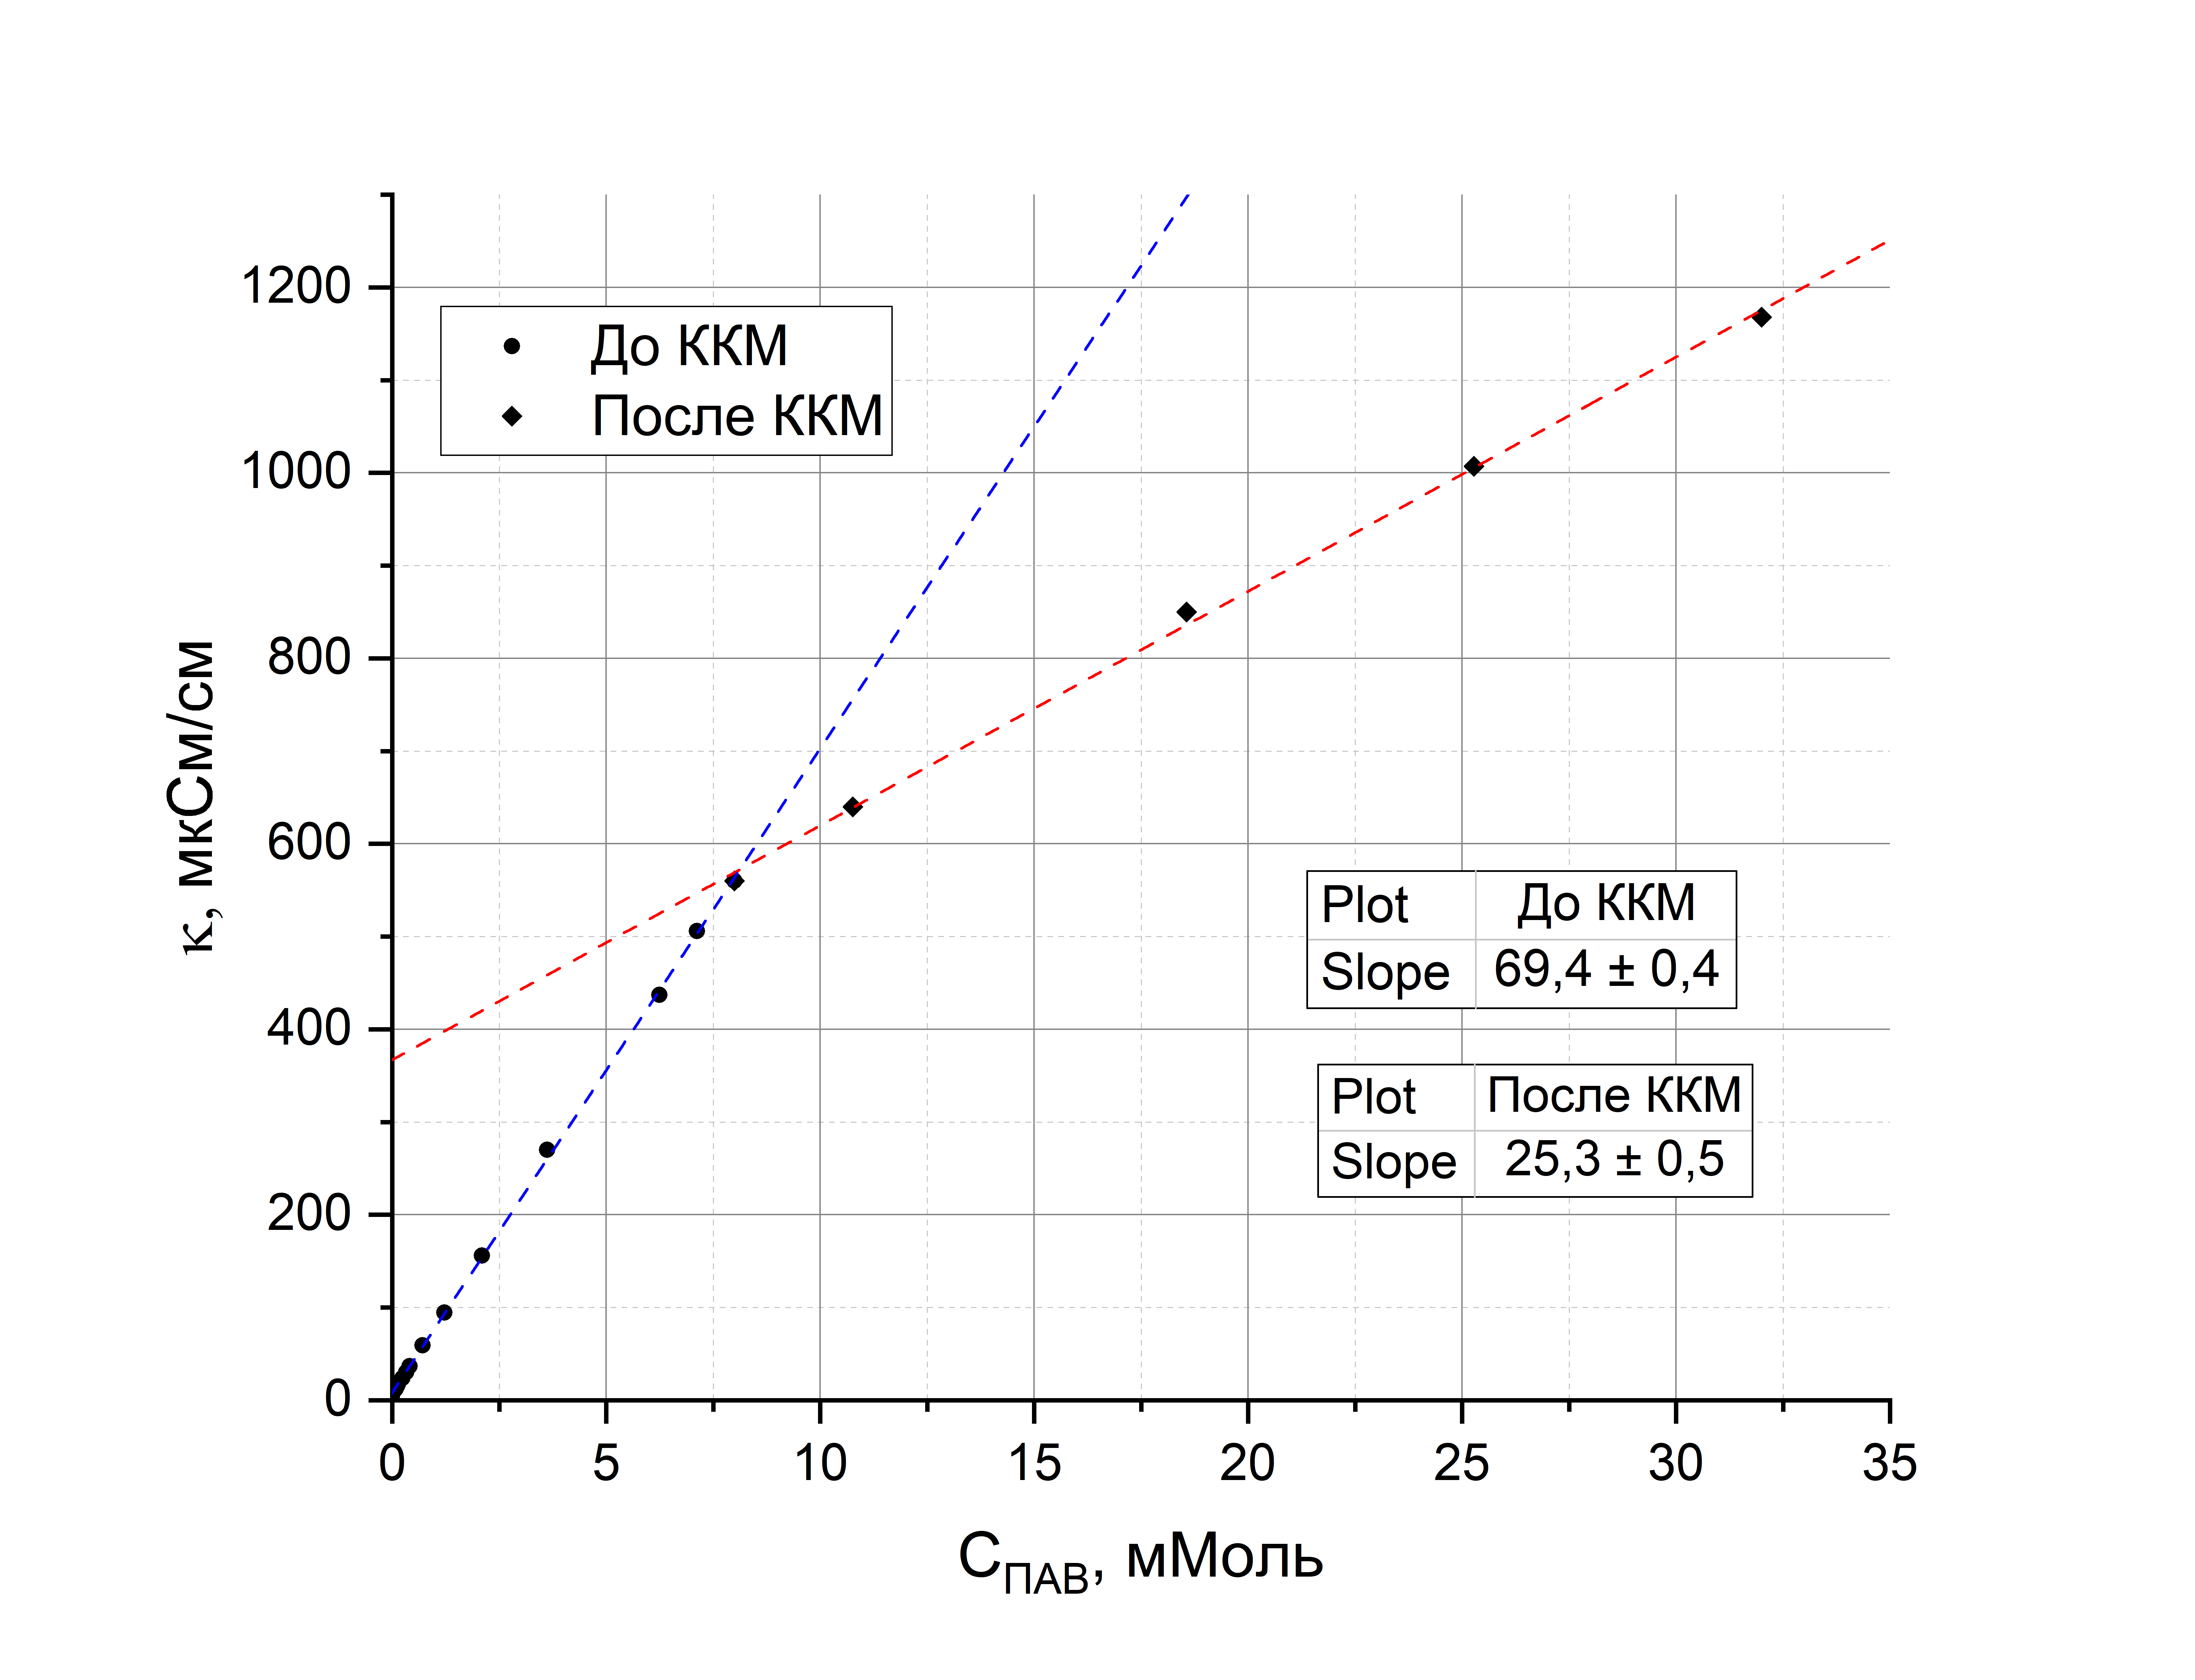
\includegraphics[width=1\textwidth]{conduct.png}
    \end{center}
    \caption{График ависимости $\kappa(C)$}
\end{figure}

По наклону графика можно оценить степень ионизации мицелл в растворе.
$$\kappa_{1}=\lambda_{N a}\left[N a^{+}\right]+\lambda_{D S}\left[D S^{-}\right]=\left(\lambda_{N a}+\lambda_{D S}\right)[S D S]$$
$$
\kappa_{2}=\lambda_{N a}\left[N a^{+}\right]+\lambda_{D S}\left[D S^{-}\right]+\lambda_{m}\left[\text { mic }^{-}\right]
$$
Используя тот факт, что 
$$
\left[D S^{-}\right]=K K M, 
\left[N a^{+}\right]=K K M+\alpha N[\text { mic }],
\left[\text { mic }^{-}\right]=\frac{[S D S]-K K M}{N}
$$
можем получить:
$$
\kappa=\alpha[S D S]\left(\lambda_{N a}+\lambda_{D S}\right)+(1-\alpha) K K M\left(\lambda_{N a}+\lambda_{D S}\right)
$$
Откуда видно что степень ионизации можно оценить как отношение наклонов линейных участков. В нашем случае $\alpha = 36.5 \pm 0.9$\%.







\subsection{Определение ККМ методом измерения поверхностного натяжения}
\subsubsection{Определение ККМ}
Сначала проведём измерения методом пластинки Вильгельми для дистиллированной воды. Поверхностное натяжение воды: $\sigma_0=72.2$мН/м. (справочное)\footnote{Никольский Б.П. Справочник химика} Т.к. $\sigma = \frac{g}{2L}\cdot{m}$, найдём "коэффициент перевода": $\frac{g}{2L}=461.55c^{-2}$. Далее проведём измерения для наших растворов. Результаты в Табл.2.

\begin{table}[h]
\begin{center}
\caption{Поверхностное натяжение растворов}
\begin{tabular}{|c|c|c|c|}
\\ \cline{1-3}
C, mM   & dm, g  & sigma   &  \\ \cline{1-3}
0       & 0.1548 & 72.2    &  \\ \cline{1-3}
0.0798  & 0.1264 & 58.3168 &  \\ \cline{1-3}
0.1349  & 0.1214 & 56.0322 &  \\ \cline{1-3}
0.2337  & 0.1313 & 60.6015 &  \\ \cline{1-3}
0.4016  & 0.1259 & 58.1091 &  \\ \cline{1-3}
0.6933  & 0.1186 & 54.7398 &  \\ \cline{1-3}
1.1953  & 0.0938 & 43.2934 &  \\ \cline{1-3}
2.0200  & 0.0869 & 40.1087 &  \\ \cline{1-3}
3.6160  & 0.0693 & 31.9854 &  \\ \cline{1-3}
6.2400  & 0.0653 & 30.1392 &  \\ \cline{1-3}
8.0000  & 0.0761 & 35.1240 &  \\ \cline{1-3}
10.7680 & 0.0818 & 37.7548 &  \\ \cline{1-3}
18.5600 & 0.0808 & 37.2932 &  \\ \cline{1-3}
32.0000 & 0.0835 & 38.5394 &  \\ \cline{1-3}
\end{tabular}
\end{center}
\end{table}

Построим графики зависимости $\sigma$ от С и $\sigma$ от lnC (c квадратичной аппроксимацией)  и определим значение ККМ по излому кривой.

\begin{figure}[h!]
\begin{center}
\begin{minipage}[h]{0.45\linewidth}
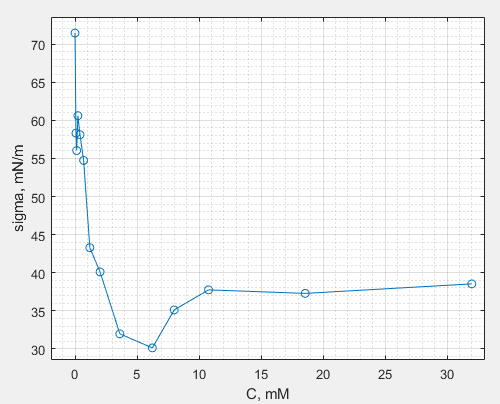
\includegraphics[width=1\textwidth]{1 sigma(C).png}
\caption{График зависимости $\sigma(C)$} %% подпись к рисунку
\label{ris:experimoriginal} %% метка рисунка для ссылки на него
\end{minipage}
\hfill 
\begin{minipage}[h]{0.5\linewidth}
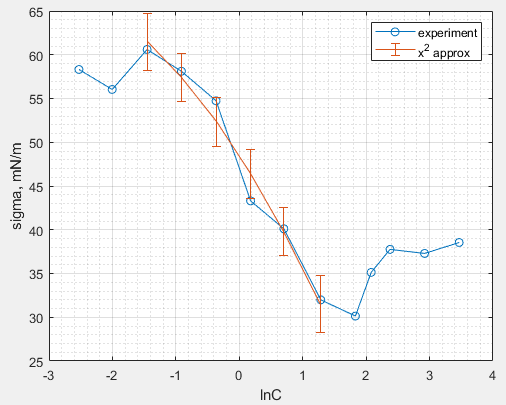
\includegraphics[width=1\textwidth]{2 sigma(lnC)+x2.png}
\caption{График зависимости $\sigma(lnC)$}
\label{ris:experimcoded}
\end{minipage}
\end{center}
\end{figure}

Из Рис.3 видим, что $lnKKM\in$[1.1, 2.4]. T.e $KKM \in$[3.0, 11.0]мМ. Определить ККМ более точно затруднительно из-за наличия примеси в растворах (минимума ниже предельного значения на графике).

\subsubsection{Определение характеристик поверхностного слоя}
Определить предельную адсорбцию можно по наклону изотермы поверхностного натяжения в конце, перед горизонтальным участком (в нашем случае - в окрестности минимума), когда формирование монослоя закончено и все вещество уходит дальше в мицеллы. 

$\left( \frac{d\sigma}{dlnC} \right) \bigg| _{\infty}$ = -13.95 мН/м.
Тогда $ \Gamma_{\infty} = \frac{-1}{RT} \cdot \left( \frac{d\sigma}{dlnC} \right) \bigg| _{\infty} = 5.63\cdot 10^{-6} \frac{mol}{m^2}$ 

По найденной предельной адсорбции определим площадь, приходящуюся на одну молекулу в плотном монослое на поверхности раствора:
$S_0 = \frac{1}{N_A \Gamma_{\infty}} = 2.95\cdot 10^{-19} \frac{m^2}{\text{шт}}$

Зная плотность раствора ПАВ: $\rho \simeq 1 g/sm^3$ и его молекулярную массу: М=288,4 a.e.м, оценим высоту молекулы в предельно плотном монослое: $l = \frac{\Gamma_{\infty}\cdot M}{\rho} = 1.62\cdot 10^{-9}m = 16.2 \buildrel _\circ \over {\mathrm{A}}$

Для оценки корректности полученного результата, сравним эту величину с оценкой по известным геометрическим размерам. Длина связи С–С в алканах около 1.5 $\buildrel _\circ \over {\mathrm{A}}$ , валентный угол $109^{\circ}$, длина связей С–H в метильной группе 2 $\buildrel _\circ \over {\mathrm{A}}$, формула для длины углеводородной цепи с n атомами углерода имеет вид: L = 1.256 (n – 1) + 2.
Для SDS(n=12): L=15.8$\buildrel _\circ \over {\mathrm{A}}$. Как видим, значение близко к оцененному из эксп.данных.

\subsubsection{Изотерма адсорбции}
Аналогично определению предельной адсорбции вычислим величины адсорбции во всех точках изотермы натяжения ($\sigma(lnC)$). Построим изотерму адсорбции Г(С) и в 1/Г(1/С), в предположении изотермы Ленгмюра: $\frac{1}{\Gamma} = \frac{1}{\Gamma_{\infty}} + \frac{1}{\Gamma \cdot K}\cdot \frac{1}{C}$. Результат на Рис. 4 и 5. 

\begin{figure}[h!]
\begin{center}
\begin{minipage}[h]{0.5\linewidth}
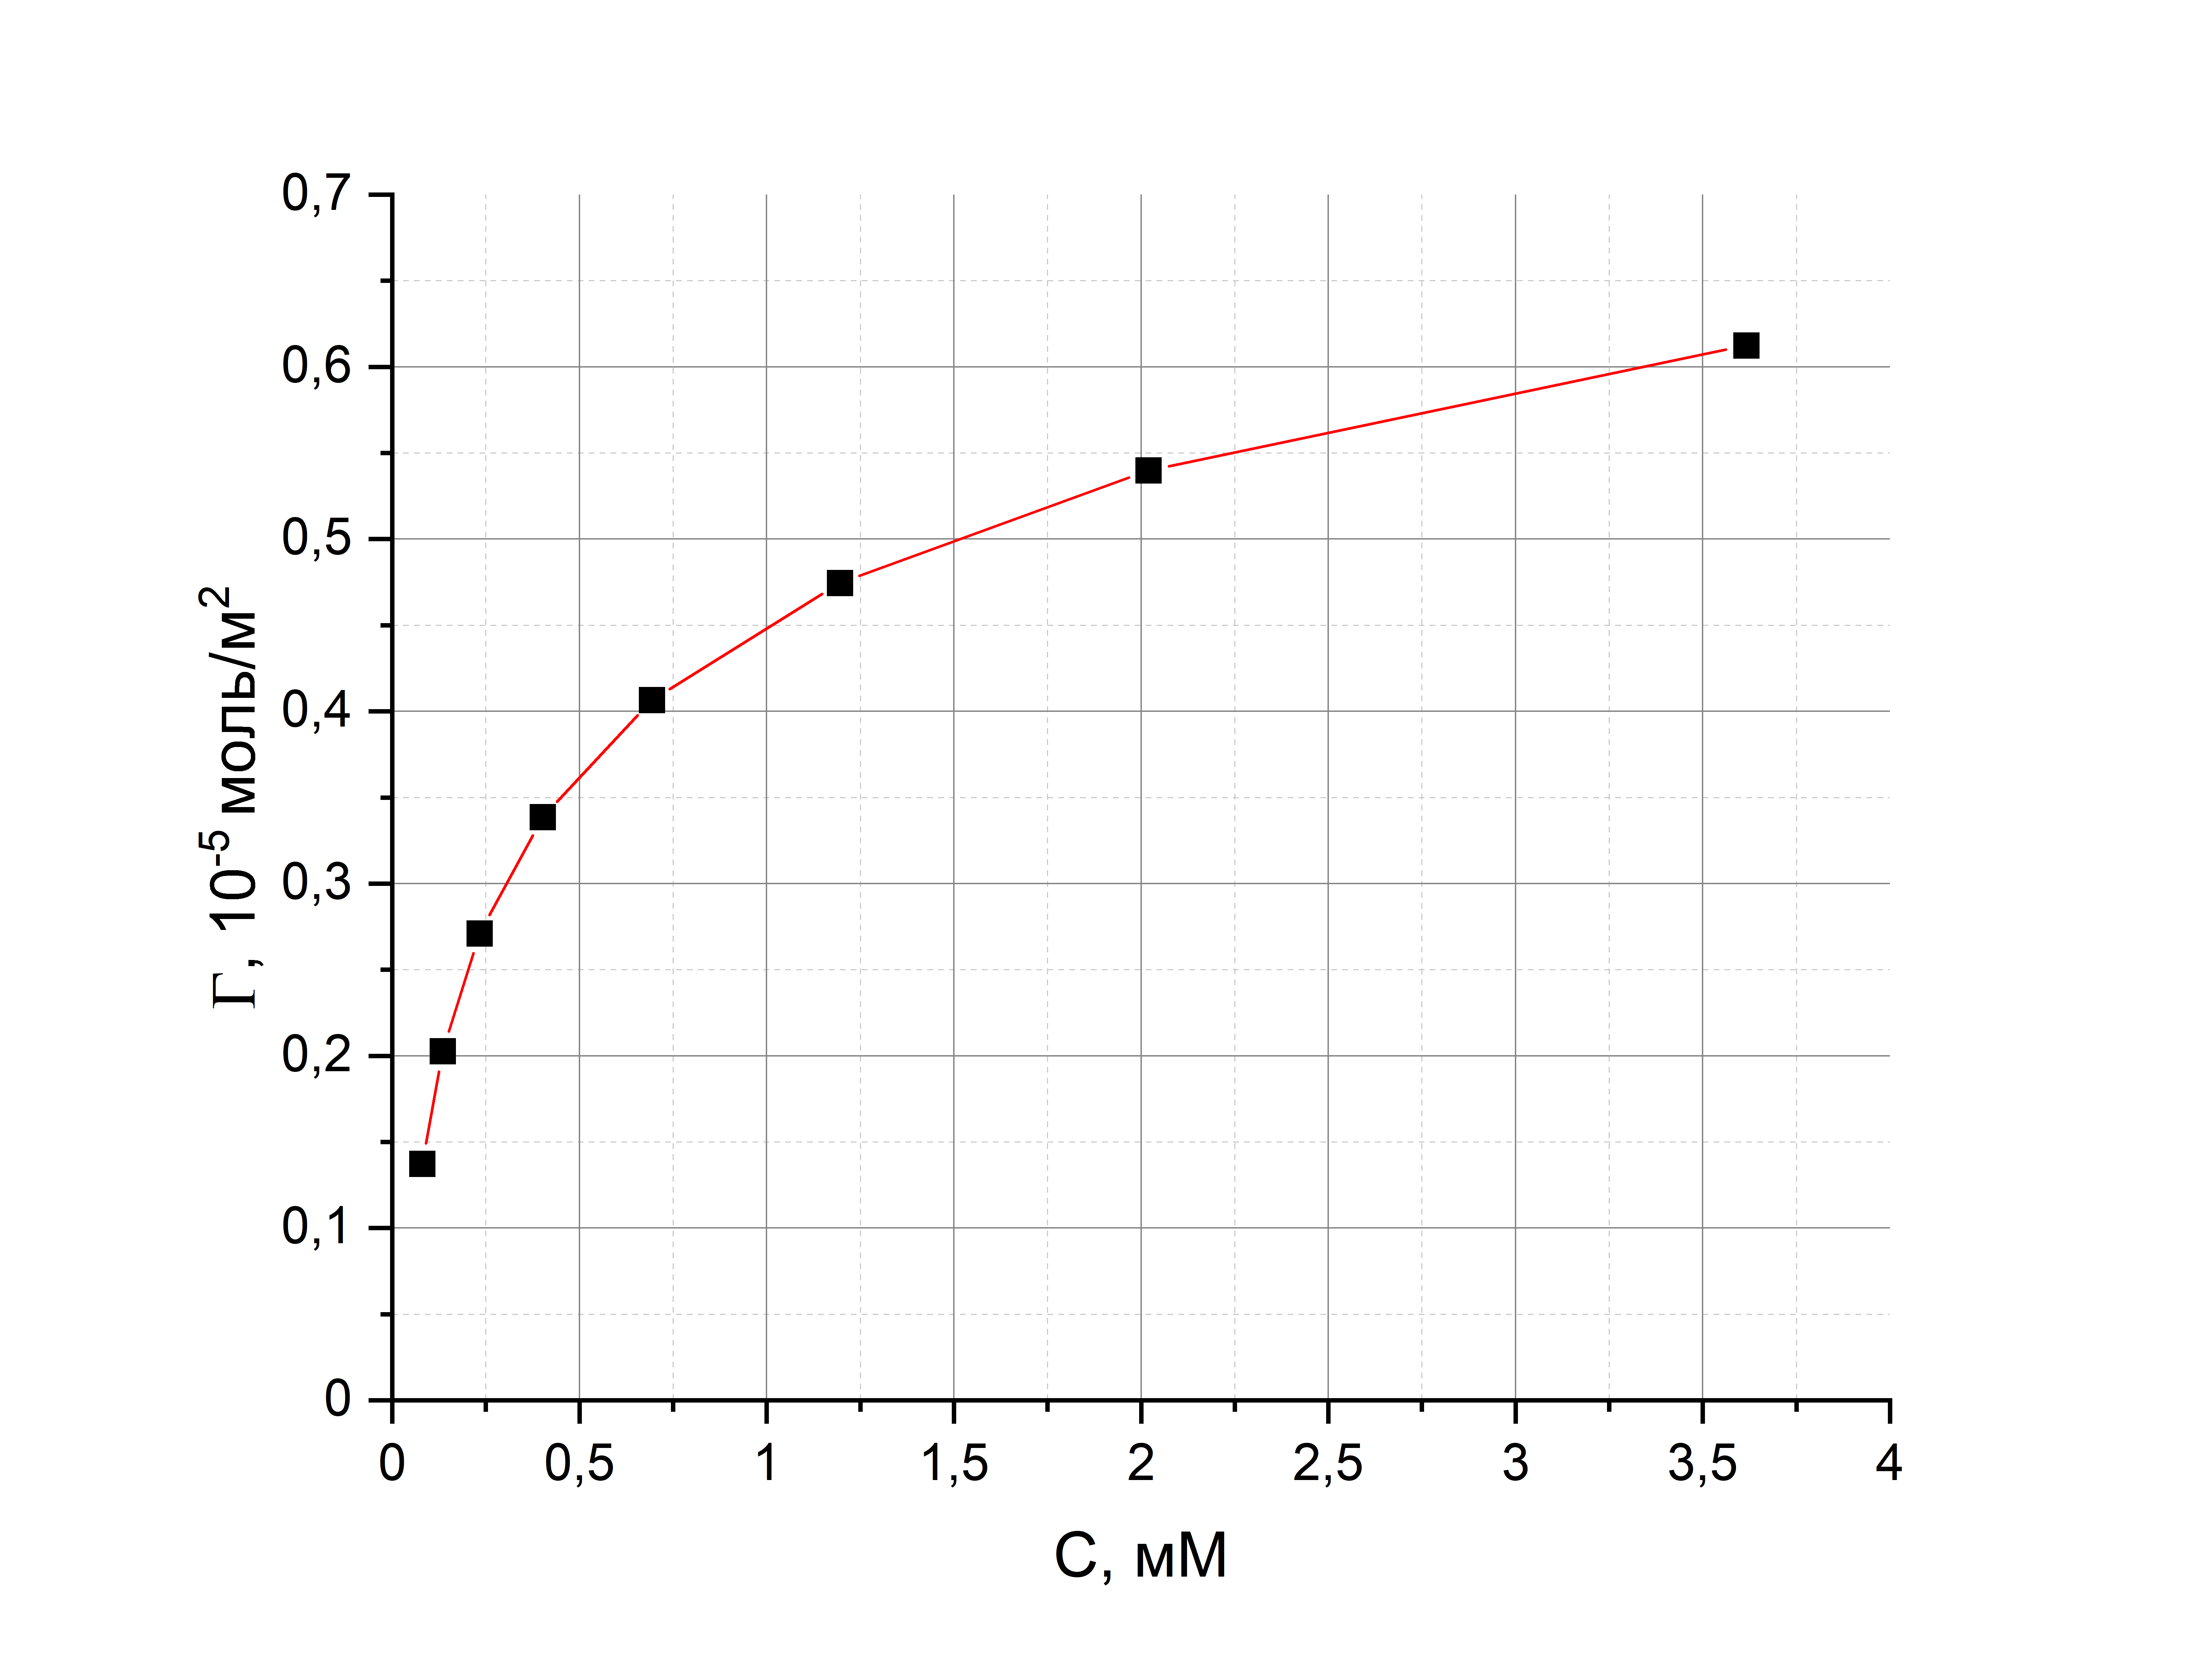
\includegraphics[width=1\textwidth]{ads.png}
\caption{Изотерма адсорбции} %% подпись к рисунку
\label{ris:experimoriginal} %% метка рисунка для ссылки на него
\end{minipage}
\hfill 
\begin{minipage}[h]{0.45\linewidth}
\includegraphics[width=1\textwidth]{4 1Г (1С).png}
\caption{Изотерма адсорбции в линеаризующих координатах}
\label{ris:experimcoded}
\end{minipage}
\end{center}
\end{figure}

По этому графику определим константу равновесия адсорбции и предельную адсорбцию: $\frac{1}{\Gamma_{\infty}} = (1.70 \pm 0.14)\cdot 10^5 \frac{m^2}{mol} \Rightarrow \Gamma_{\infty} = (5.9 \pm 0.5)\cdot 10^{-6} \frac{mol}{m^2}$ 

$\frac{1}{K \Gamma_{\infty}} = (44.7 \pm 2.6) \frac{m^2}{M*mol} \Rightarrow K = (3.8 \pm 0.3)\cdot 10^3 \frac{1}{M}$
Видим, что $\Gamma_{\infty}$, определённая по изотерме адсорбции и изотерме поверхностного натяжения, совпадают в пределах погрешности.

\subsubsection{Определение станд. своб. энергии адсорбции}
Зная константу адсорбции, получим стандартную свободную энергию адсорбции: $\Delta G = -RTlnK = (-20.41 \pm 0.25)$кДж/моль. 

По правилу Траубе $\frac{g_{n+1}}{g_n} = \frac{\Gamma_{n+1}}{\Gamma_n} = \frac{K_{n+1}}{K_n} = \alpha = 2.1$ (для ионогенных ПАВ). (Т.к. $g_n = -\frac{d\sigma}{dC} \bigg| _{c->0}$ , a $\Gamma_{\infty}$ одинакова для всех гомологов). Тогда $\Delta G_{n+1} - \Delta G_n = -RTln \alpha$. И можем оценить $\Delta G^0_{12} \sim -12 RT ln \alpha \simeq -22$ кДж/моль. Как видим, значение близко к значению, посчитаному по определению.


%%%%%%%%%%%%%%%%%%%%%%%%%%%%%%%%%%%%%%%%%%%%%%%%%%%%%%%%%%%%%%%%%%%%%%%%%
 \section{Выводы}
\begin{enumerate}
    \item На примере кондуктометрических измерений было возможно убедиться в резком изменении свойств раствора при пересечении ККМ по концентрации. Оба участка графика были линейны, благодря чему относительно точно была посчитана величина ККМ - 8.1 против 8.2 мМ согласно справочным данным. Также в простейшей оценке была получена степень ионизации $\alpha = 36$\%.
    
    \item Тензиометрическим методом получена зависимость поверхностного натяжения от концентрации раствора ПАВ. Определить по ней ККМ можно только с существенно более низкой точностью из-за наличия примеси. 
    
    \item Построена изотерма адсорбции. По ней определены предельная адсорбция, константа адсорбции, станд.своб.энегрия адсорбции. По величине предельной адсорбции оценены площадь на одну молекулу и её высота в предельно насыщенном слое. 

\end{enumerate}

\end{document}
